\documentclass{article}

\usepackage{color}
\usepackage{graphicx}
\usepackage{wrapfig}

\title{\textbf{\textcolor{red}{My Role Model-Kazi Nazrul Islam}}}
\author{\textbf{\textbf{Shuvasish Karmaker-0705008}}}
\date{September 19,2010}

\begin{document}
\maketitle
\section*{\textcolor{magenta} {\textbf{\LARGE{{Introduction}}}}} 




\begin{wrapfigure}{r}{0.55\textwidth}
\vspace{-10pt}

\begin{center}
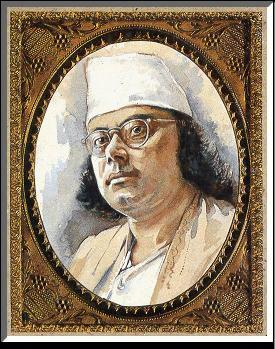
\includegraphics[width=.45\textwidth]{pic1}
\end{center}

\vspace{-10pt}
\caption{Kazi Nazrul Islam (1898-1976)}
\vspace{-10pt}
\end{wrapfigure}



\textbf{\textit{Kazi Nazrul Islam}} Islam was born in the village of \textcolor{blue}{Churulia} in the Burdwan District of Bengal (now located in the Indian state of West Bengal).He was born in a Muslim family who is second of three sons and a daughter, Nazrul's father \textcolor{blue}{Kazi Fakeer Ahmed} was the imam  and caretaker of the local mosque and mausoleum. Nazrul's mother was \textcolor{blue}{Zaheda Khatun}. Nazrul had two brothers, Kazi Shahebjan and Kazi Ali Hussain, and a sister, Umme Kulsum. Nicknamed \textbf{\textit{Dukhu Mia}} (Sad Man), Nazrul began attending the maktab � the local religious school run by the mosque � where he studied the Qur'an and other scriptures, Islamic philosophy and theology. His family was devastated with the death of his father in 1908. 



\section*{\textcolor{magenta} {\textbf{\LARGE{{Rebel Poet}}}}}

Nazrul left the army in 1920 and settled in Calcutta, which was then the Cultural capital of India (it had ceased to be the political capital in 1911).He joined the staff of the \textcolor{blue}{�Bangiya Mussalman Sahitya Samiti�}  and roomed at 32 College Street  with colleagues. He published his first novel \textcolor{blue}{"Bandhan-hara" ("Freedom from bondage")} in 1920, which he kept working on over the next seven years. is first collection of poems included \textbf{\textit{"Bodhan"}}, \textbf{\textit{"Shat-il-Arab"}}, \textbf{\textit{"Kheya-parer Tarani"}} and \textbf{\textit{"Badal Prater Sharab"}} and received critical acclaim.





\begin{wrapfigure}{r}{0.4\textwidth}
\vspace{-10pt}

\begin{center}
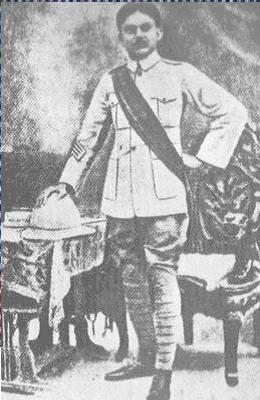
\includegraphics[width=0.40\textwidth]{pic2}
\end{center}

\vspace{-10pt}
\caption{Nazrul in Army}
\vspace{-10pt}
\end{wrapfigure}






\section*{\textcolor{magenta} {\textbf{\LARGE{{Later life and Illness}}}}}

Nazrul's success soon brought him into Indian theatre and the then-nascent film industry. The first picture for which he worked was based on Girish Chandra Ghosh's story \textcolor{blue}{"Bhakta Dhruva"} in 1934.The film "Vidyapati" ("Master of Knowledge") was produced based on his recorded play in 1936, and Nazrul served as the music director for the film adaptation of Tagore's novel \textcolor{blue}{Gora}. He produced critical and analytic documentaries on music, such as \textcolor{blue}{"Haramoni"} and \textcolor{blue}{"Navaraga-malika"}.  He Sought to preserve his artistic integrity by condemning the adaptation of his songs to music composed by others and insisting on the use of tunes he composed himself.








\section*{\textcolor{magenta} {\textbf{\LARGE{{Why Kazi Nazrul Islam is my role model?}}}}} 

The word \textcolor{blue}{role model} implies that  \textcolor{red}{"any person who deserves as an example, whose behaviour is praised by others,who is followed by others"}. Since, it is very easy to find out the qualities of that person you like most, i only focus the behaviour which attracts me most .No doubt \textbf{\textit{Kazi Nazrul Islam}}'s extra-ordinary talent in Bangla literature has made me attractive to him and he is placed in the Heart of mine.




\end{document}



